\documentclass[12pt,a4paper]{article}

\usepackage[utf8]{inputenc}
\usepackage[english]{babel}
\usepackage{amsmath}
\usepackage{amsfonts}
\usepackage{amssymb}
\usepackage{makeidx}
\usepackage{graphicx}
\usepackage{subcaption}
\usepackage{caption}
\usepackage{float}
\usepackage[left=2cm,right=2cm,top=2cm,bottom=2cm]{geometry}
\usepackage{tikz}
\usepackage{pdfpages}
\pagestyle{plain}
\usepackage{bm}
\usepackage{ulem}
\usepackage{units}
\usepackage{makecell}

%Kopf und Fußzeile:
\usepackage{fancyhdr}
\pagestyle{fancy}
\fancyhf{}
\renewcommand{\footrulewidth}{0.4pt}
\usepackage{array}   % for \newcolumntype macro
\newcolumntype{C}{>{$}c<{$}} % math-mode version of "c" column type

\fancyhead[L]{Computational photonics}
%\fancyhead[C]{Dr. Bj\"orn Leder}
\fancyhead[R]{Excercise 1}
\fancyfoot[L]{\today}
\fancyfoot[R]{page \thepage}
\fancyfoot[C]{Julien Kluge}

% Code-Listings
\usepackage{listings}
\lstset{
language=c,
showstringspaces=false,
numbers=left,
xleftmargin=2em}

% Ganze Dateien als Verbatim einbinden
%\usepackage{verbatimfiles} % downloaded from ctan.org

\title{Computational photonics}
\author{Julien Kluge}
\date{\today}

%============================================================
% Dokument
%============================================================
\begin{document}

\lstset{numbers=left}

\begin{center}
\large{\textbf{Computational photonics -- Excercise 1}} \\
~\\
\small{-- Julien Kluge (564513) --}\\
~\\
Date: \today
\end{center}
\hrule


\section*{Task 1}
	\begin{table}[H]
		\caption{Program file index - Task 1}
		\begin{tabular}{r|c|l}
			\textit{A1/A1.m} & Matlab & program with whole task in sections
		\end{tabular}
	\end{table}
	\subsection*{a)}
		\begin{lstlisting}
gauss1D = @(x) exp(-(x * x));
x = -xMax:dx:xMax;
y = arrayfun(gauss1D, x);
plot(x, y)
		\end{lstlisting}
		\begin{figure}[H]
			\centering
			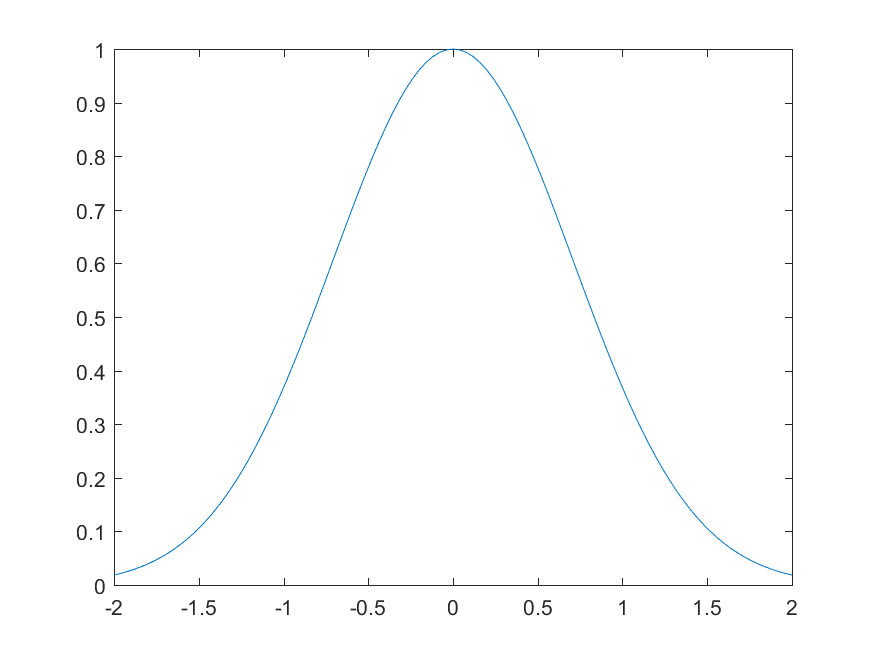
\includegraphics[width=0.7\textwidth]{A1/A1_a.png}
			\caption{Plot of the function \(f(x)=\exp\left(-x^2\right)\) in matlab.}
		\end{figure}
	\subsection*{b)}
		\begin{lstlisting}
gauss2D = @(x, y) exp(-(x * x + y * y));
g = -gMax:dg:gMax;
[x, y] = meshgrid(g, g);
z = arrayfun(gauss2D, x, y);
mesh(x, y, z)
surface(x, y, z)
pcolor(x, y, z)
contour(x, y, z)
		\end{lstlisting}
		\begin{figure}[H]
			\centering
			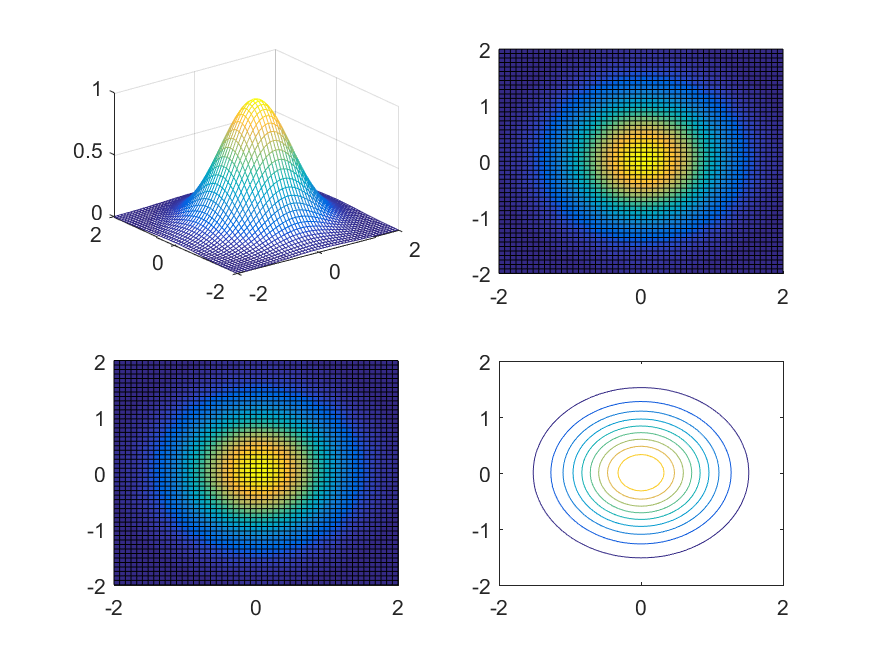
\includegraphics[width=0.9\textwidth]{A1/A1_b.png}
			\caption[]{Plot of the function
			\(f(x)=\exp\left(-\left(x^2+y^2\right)\right)\) in matlab for different commands.}
		\end{figure}
	\subsection*{c)}
		Quiver code omitted for clarity in this document.
		\begin{figure}[H]
			\centering
			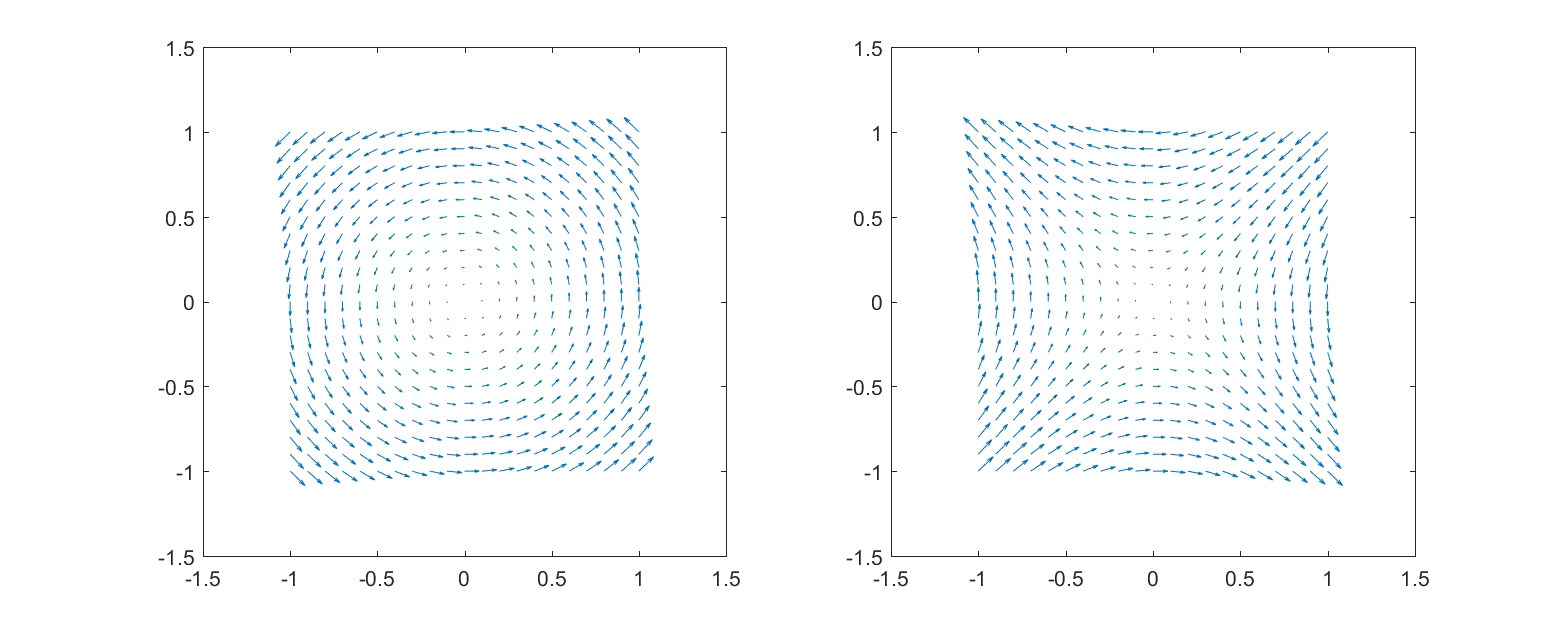
\includegraphics[width=\textwidth]{A1/A1_c.png}
			\caption[]{Vectorfields \(\mathbf{E_1}=(-y, x)\) and \(\mathbf{E_2}=-(y, x)\) plotted with quiver.}
		\end{figure}
	\subsection*{d)}
		\begin{lstlisting}
	h = @(x) exp(1 - 1 ./ x) ./ x;
	int1 = integral(h, eps, 1);
		\end{lstlisting}
		\begin{figure}[H]
			\centering
			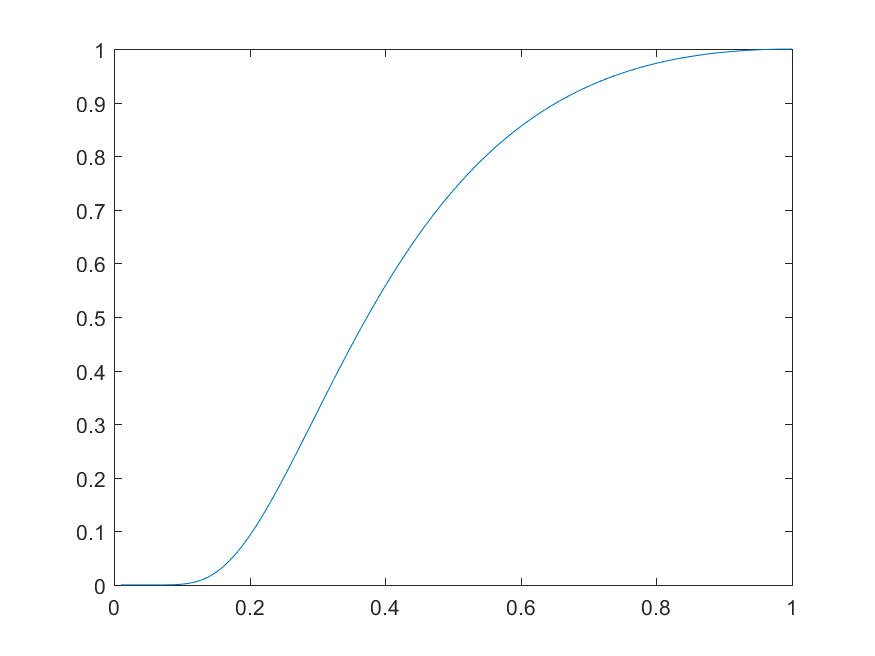
\includegraphics[width=0.7\textwidth]{A1/A1_d.png}
			\caption[]{Function \(h(x)\) plotted in matlab.}
		\end{figure}
		Even though matlab properly integrates this function and acquires
		the right value of about
		\begin{align}
			\int_0^1\text{d}x\,h(x)=e\cdot\Gamma\left(0,1\right)\approx 0.5963
		\end{align}
		it could still pose a problem for similar functions since the function
		inhibits a pole on \(x=0\). It can easily through variable substitution be shown,
		that
		\begin{align}
			\lim_{x\rightarrow 0}h(x)=0
		\end{align}
		but programs cannot do the symbolic limit implicitly and therefore acquire an error
		due to the division by zero. This can be cirumvented with two possibilities:
		\begin{enumerate}
			\item Since we know \(h(x\rightarrow0)\rightarrow0\) we can explicitly spare the
			integral-function of the pole by adjusting integration limit to \(\left[\epsilon,1\right]\)
			where \(\epsilon\) is the machine-epsilon of the according floating point type (\textit{eps} in matlab).
			\item We can do a variable substition \(x=1/y\) under the integral
			\begin{align}
				\int_0^1\text{d}x\,\frac{\exp\left(1-\frac{1}{x}\right)}{x}=\int_1^\infty\text{d}y\,\frac{\exp\left(1-y\right)}{y}
			\end{align}
			This seems to pose the exchanged problem of integrating to infinity. However, after quick
			calculations in can be shown that \(h(y)<\epsilon\) for \(y\geq 34.31\) with a
			strong monotonic descrease (\(h(y)\propto1/\left(y\cdot\exp y\right)\)). So we can comfortably
			set the integration limits to \([1,34.31]\) (or adapting to a specific precision-limit).
		\end{enumerate}
		\newpage

\section*{Task 2}
	\begin{table}[H]
		\caption{Program file index - Task 2}
		\begin{tabular}{r|c|p{10cm}}
			\textit{A2/A2.jl} & Julia & program with tasks a, b and part of c \\
			\textit{A2/naiveDFT.jl} & Julia & implementation of the naive dft in matrix and\newline iterative form \\
			\textit{A2/simpleDFT.jl} & Julia & implementation of the recursive dft \\
			\textit{A2/benchmarkFunction.jl} & Julia & benchmark function for fft-functions \\
			
			\textit{A2/A2c\_MatlabFFT.m} & Matlab & programm to acquire matlab fft benchmarks \\
			\textit{A2/A2d.nb} & Mathematica & notebook to calculate aliasing graphs \\
			\textit{A2/data/Visualize.nb} & Mathematica & notebook to calculate graphs for c
		\end{tabular}
	\end{table}
	\subsection*{a) and b)}
		According to the program file index the ffts where implemented in naive and recursive
		form and compared to the FFTW package. The comparison was made with an artificial created
		dataset of three sine waves with different amplitude, frequency and phase.
		\begin{figure}[H]
			\centering
			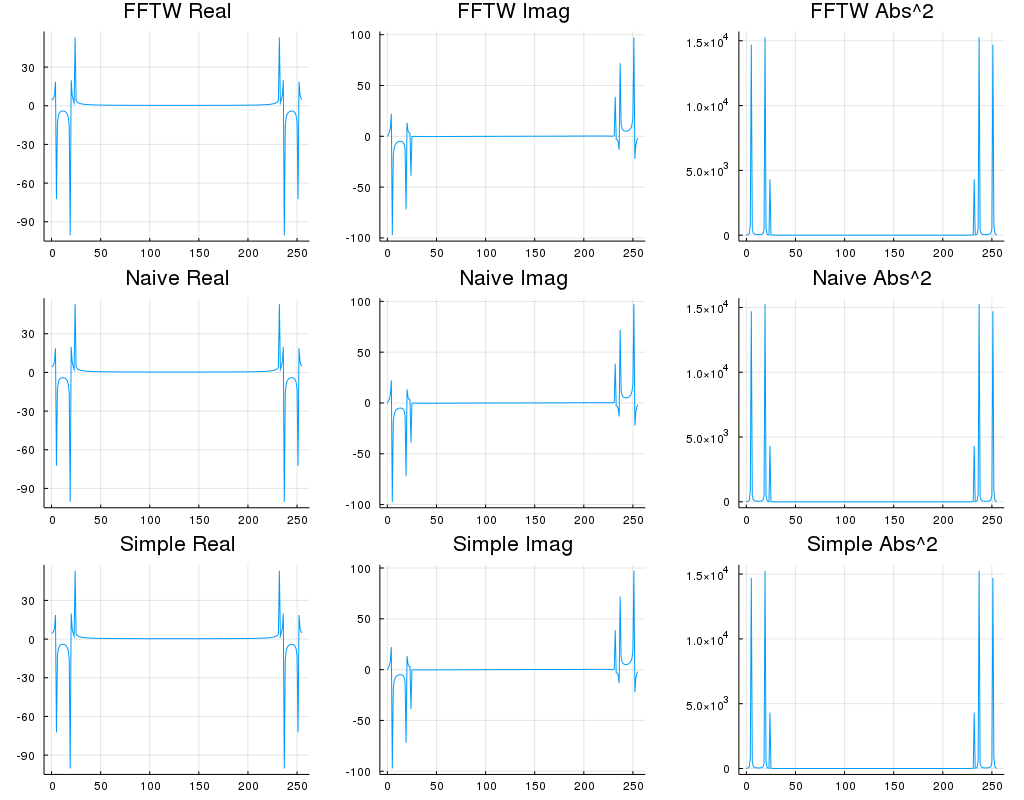
\includegraphics[width=\textwidth]{A2/data/fftPlot.png}
			\caption[]{Comparison of real, imaginary and absolute values of FFTW, the naive and recursive implementation}
		\end{figure}
		The summed differences where all calculated to be below \(10^{-10}\).
	
	\subsection*{c)}
		The Julia functions and a Matlab benchmark where made with different problem sizes
		all with a power of two. The stopping criterion was set, when an implementation
		reached calculation times over a second. Each test was repeated five times and
		was averaged out.\\
		Following results where acquired:
		\begin{figure}[H]
			\centering
			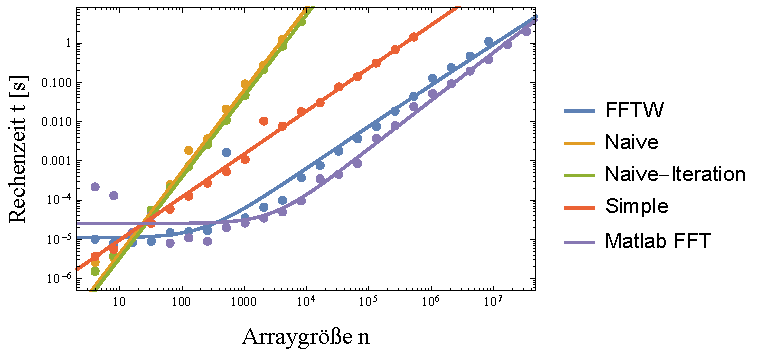
\includegraphics[width=0.7\textwidth]{A2/data/Comparison.pdf}
			\caption[]{Comparisons between different dft implementations. The simple, recursive
			Julia implementation is notably only 5 times slower than FFTW.}
		\end{figure}
		The fastest implementation seems to be matlabs fft. However, it is known
		that matlab utilizes FFTW-plan implementations. The exact same speed could
		be therefore in Julia be acquired with a single FFTW-plan allocation.\\
		The naive implementations are fitted with a runtime slightly above
		\(\mathcal{O}\left(N^2\right)\). All other implemntations are approximately
		\(\approx\mathcal{O}\left(N^{1.1}\right)\) for the simple, recursive implementation
		and \(\mathcal{O}\left(N\log N\right)\) in the given uncertainty intervals.

	\subsection*{d)}
		\begin{align}
			\hat{\mathcal{F}}_t^\omega\left\{\exp\left(-t^2\right)\right\}=\sqrt{\pi}\exp\left(\frac{-\omega^2}{4}\right)
		\end{align}
		\begin{figure}[H]
			\centering
			\begin{subfigure}[b]{0.45\textwidth}
				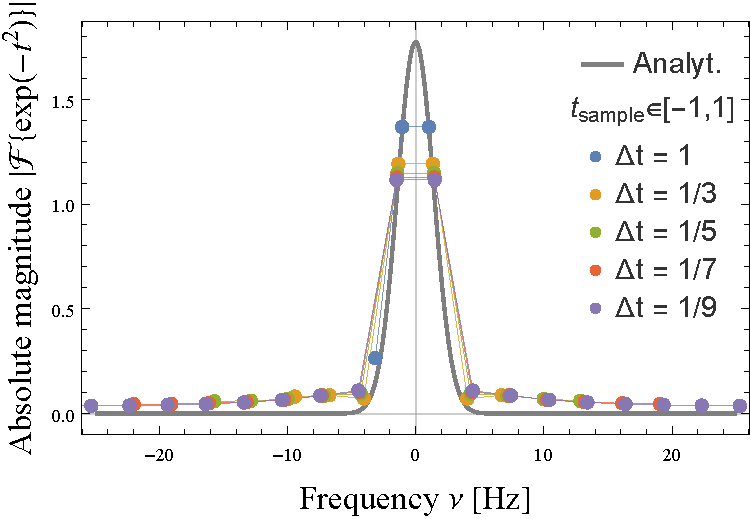
\includegraphics[width=0.9\columnwidth]{A2/data/DT_Comparison.pdf}
				\caption[]{Comparison between different sampling distances \(\Delta t\)}
			\end{subfigure}
			\begin{subfigure}[b]{0.45\textwidth}
				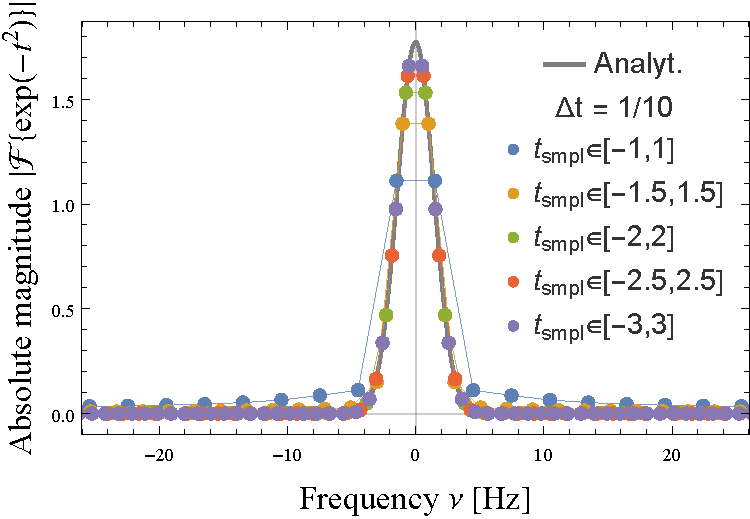
\includegraphics[width=0.9\columnwidth]{A2/data/TSampling_Comparison.pdf}
				\caption[]{Comparison between different sampling intervals \(t_{smpl}\in\left[-t, t\right]\)}
			\end{subfigure}
			\caption[]{Comparison of aliasing in different sample intervals and sampling distances.}
		\end{figure}
		\noindent It can quickly be seen how the different intervals and distances distort the resulting
		fourier points. The sampling interval seems to have a stronger effect.\\
		To confirm that, a density plot of the absolute differences to the analytical solution
		can be made.
		\begin{figure}[H]
			\centering
			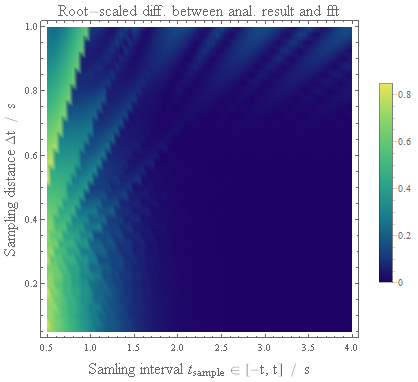
\includegraphics[width=0.7\textwidth]{A2/data/DT_TSampling_Contour.png}
			\caption[]{Absolute differences of fft to analytical solution, scaled
			by the squareroot (for better visibility) in respect to the sampling
			interval and distances.}
		\end{figure}
		\noindent The multiplication by \(N\,\Delta t\, (-1)^n\) is necessary to
		normalize the fourier coefficients and the last term is for shifting the resulting
		coefficients to the zero-frequency.
		\newpage
	
\section*{Task 3}
	\begin{align}
		\frac{\partial \mathbf{H}(\mathbf{r,t})}{\partial t}&=-\frac{1}{\mu_0\,\mu(\mathbf{r})}\nabla\times\mathbf{E}(\mathbf{r},t)\\
		\frac{\partial \mathbf{E}(\mathbf{r,t})}{\partial t}&=\frac{1}{\epsilon_0\,\epsilon(\mathbf{r})}\nabla\times\mathbf{H}(\mathbf{r},t)
	\end{align}
	First we introduce to arbitrary field strengths \(E_0, H_0\) such that
	\begin{align}
		\frac{\mathbf{E}}{E_0}&=\widetilde{\mathbf{E}} \\
		\frac{\mathbf{H}}{H_0}&=\widetilde{\mathbf{H}}
	\end{align}
	Which then renders the upper equations to
	\begin{align}
		\frac{\partial \widetilde{\mathbf{H}}(\mathbf{r,t})}{\partial t}&=-\frac{E_0}{H_0\,\mu_0}\frac{1}{\mu(\mathbf{r})}\nabla\times\widetilde{\mathbf{E}}(\mathbf{r},t)\\
		\frac{\partial \widetilde{\mathbf{E}}(\mathbf{r,t})}{\partial t}&=\frac{H_0}{E_0\,\epsilon_0}\frac{1}{\epsilon(\mathbf{r})}\nabla\times\widetilde{\mathbf{H}}(\mathbf{r},t)
	\end{align}
	We can equate the terms with \(E_0,H_0,\epsilon_0,\mu_0\) to a constant.
	Since the field strength modifier are arbitrary, the constants are also arbitrary.
	Therefore we set it equal to one:
	\begin{align}
		1&=\frac{E_0}{H_0\,\mu_0} \\
		1&=\frac{H_0}{E_0\,\epsilon_0}
	\end{align}
	This system is underdetermined. We can therefore only solve for one solution.
	Multiplication and division yields following equations respectively
	\begin{align}
		1&=\frac{1}{\epsilon_0\,\mu_0}=c^2 \\
		1&=\frac{E_0^2\,\epsilon_0}{H_0^2\,\mu_0}
	\end{align}
	The first gives the natural units where \(c=1\). This enables further manipulation
	for time or space such that \(\mathbf{r}/r_0=\widetilde{\mathbf{r}}\) and
	\(t\cdot c/r_0=\widetilde{t}\). The second equation gives a solution for either variable.
	For the arbitrary decision to solve \(H_0\) we get
	\begin{align}
		H_0=E_0\sqrt{\frac{\epsilon_0}{\mu_0}}
	\end{align}
	Thus the final result in natural units (\(c=1\)) can be archived:
	\begin{align}
		\frac{\partial \widetilde{\mathbf{H}}(r_0\,\widetilde{\mathbf{r}},r_0\,\widetilde{t})}{\partial \widetilde{t}}&=-\frac{1}{\mu(r_0\,\widetilde{\mathbf{r}})}\nabla_{\widetilde{r}}\times\widetilde{\mathbf{E}}(r_0\,\widetilde{\mathbf{r}},r_0\,\widetilde{t})\\
		\frac{\partial \widetilde{\mathbf{E}}(r_0\,\widetilde{\mathbf{r}},r_0\,\widetilde{t})}{\partial \widetilde{t}}&=\frac{1}{\epsilon(r_0\,\widetilde{\mathbf{r}})}\nabla_{\widetilde{r}}\times\widetilde{\mathbf{H}}(r_0\,\widetilde{\mathbf{r}},r_0\,\widetilde{t})
	\end{align}
	Which also gives us the spatial discretization as \(r_0\).
\end{document}
